\documentclass{article}

\usepackage{tikz}
\usetikzlibrary{positioning, fit,  shapes.geometric}
\usepackage{ifthen}
\usepackage{etoolbox}

\tikzset{
	backgroundcolor/.style ={fill=white},
	every node/.append style={
		minimum height=7mm,
	},
	labe/.append style={
		%Blue,
		align = center,
		backgroundcolor,
		fill opacity=0.6,
		text opacity=1,
		font={\footnotesize\itshape}	
	},
	layer/.append style={
		draw,
		align = center,
		minimum height=7mm,
	},
	tight/.append style={
		inner sep=0.2mm,
	},
	lookupbox/.append style={
		draw=none,
		append after command={
		       	[shorten <= -0.5\pgflinewidth]
		       	([shift={(-1.5\pgflinewidth,-0.5\pgflinewidth)}]\tikzlastnode.north east)
		       	edge([shift={( 0.5\pgflinewidth,-0.5\pgflinewidth)}]\tikzlastnode.north west) 
		       	([shift={( 0.5\pgflinewidth,-0.5\pgflinewidth)}]\tikzlastnode.north west)
		       	edge([shift={( 0.5\pgflinewidth,-1.5\pgflinewidth)}]\tikzlastnode.south west)            
		       	([shift={( -1.5\pgflinewidth,+0.5\pgflinewidth)}]\tikzlastnode.south east)
		       	edge([shift={(-1.5\pgflinewidth,-0.5\pgflinewidth)}]\tikzlastnode.north east)
		},
		inner sep=0.7mm,
		outer sep=0mm,
		minimum width=25mm
	}
}

\begin{document}

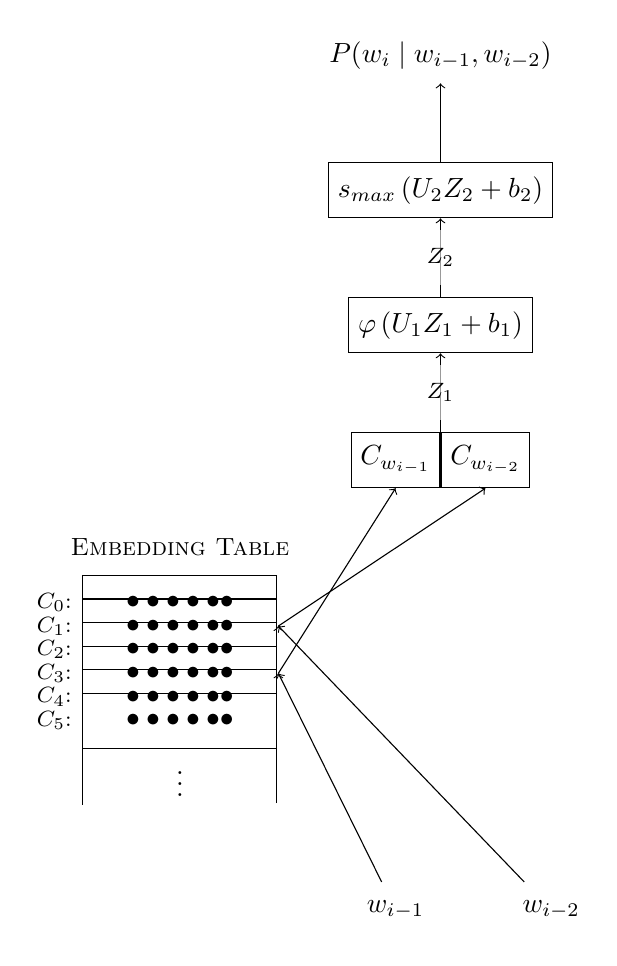
\begin{tikzpicture}[]


\node(w1) {$w_{i-1}$};
\node(w2)[right = of w1] {$w_{i-2}$};


\node(Cn)[lookupbox, above left=of w1] {$\vdots$};
\def\tblmax{6}
\foreach \ii in {1,...,\tblmax} {
	\pgfmathsetmacro\pos{(\ii - 1) * 3 };
	\pgfmathtruncatemacro\jj{(\tblmax -\ii)};
	
	\node(C\ii)[lookupbox, above = \pos mm of Cn]{$\bullet\bullet\bullet\bullet\bullet\bullet$};
	\node(Clbl\ii)[left = 0mm of C\ii]{\footnotesize $C_\jj$:};
};
\node(C)[above = 0mm of C\tblmax] {\small \textsc{Embedding Table}};


\node(concat1)[layer, above = 5 of w1]{$C_{w_{i-1}}$};
\node(concat2)[layer, right = 0 of concat1]{$C_{w_{i-2}}$};

\draw[->] (w1) edge (C3.east);
\draw[->]  (C3.east) edge (concat1.south);
\draw[->] (w2) edge (C5.east);
\draw[->]  (C5.east) edge (concat2.south);

\node(L1)[layer, above = of concat1.north east]{$\varphi\left(U_1Z_1 + b_1\right)$};
\draw[->]  (concat1.north east) -- node[labe]{$Z_1$} (L1);

\node(L2)[layer, above = of L1]{$s_{max}\left(U_2 Z_2 + b_2\right)$};
\draw[->]  (L1) edge node[labe]{$Z_2$} (L2);

\node(out)[above = of L2]{$P(w_i \mid w_{i-1}, w_{i-2})$};
\draw[->] (L2) edge (out);
\end{tikzpicture}

\end{document}